\chapter{Introdução}\label{introducao}
% determinacao da potencia sonora
Várias técnicas de controle de ruído foram desenvolvidas nesses últimos tempos visando oferecer ao ouvido humano um ambiente agradável, principalmente no que diz respeito a filtragem em determinadas faixas de frequências. Para tanto, faz-se uso de filtros acústicos de natureza mecânica.

Para a determinação dos procedimentos de medição da perda de transmissão de filtros acústicos tomasse como referência a norma ASTM E2611 – 9 Standard Test Method for Measurement of Normal Incidence Sound Transmission of Acoustical Materials Based on the Transfer Matrix Method. Os procedimentos descritos nessa norma abrange a utilização de um tubo, quatro microfones, um hardaware para aquisição do sinal em níveis de pressão e um software de análise de sinal para a determinação das funções de transferência e outras propriedades acústicas relevantes.

Em vista do que foi exposto, esse trabalho tem como objetivo determinar e analisar o comportamento da absorção acústica em dois tipos de filtros acústico: câmara de expansão e ressonador de Helmholtz.

\chapter{Fundamentação Teórica}\label{fundamentacao}


\chapter{Experimento e Equipamentos}\label{descricao}

Para realizar as medições utilizou-se os seguintes instrumentos:

\begin{itemize}
	\item dois microfones;
	\item um calibrador de microfone;
	\item dois rotating boom;
	\item um computador
	\item um analisador de sinais modelo SCADAS da LMS;
	\item uma placa de teste (1800 mm x 1130 mm x 2 mm);
	\item uma fonte sonora;
	\item um amplificador de potência;
	\item uma fonte Sonora de referência.
\end{itemize}

E o esquemático das câmaras I e II, geradora e receptora respectivamente, foi constituída de acorda com a figura \ref{experimento_1}.

\begin{figure}[h]
	\centering
	%\hspace{-4.5cm}
	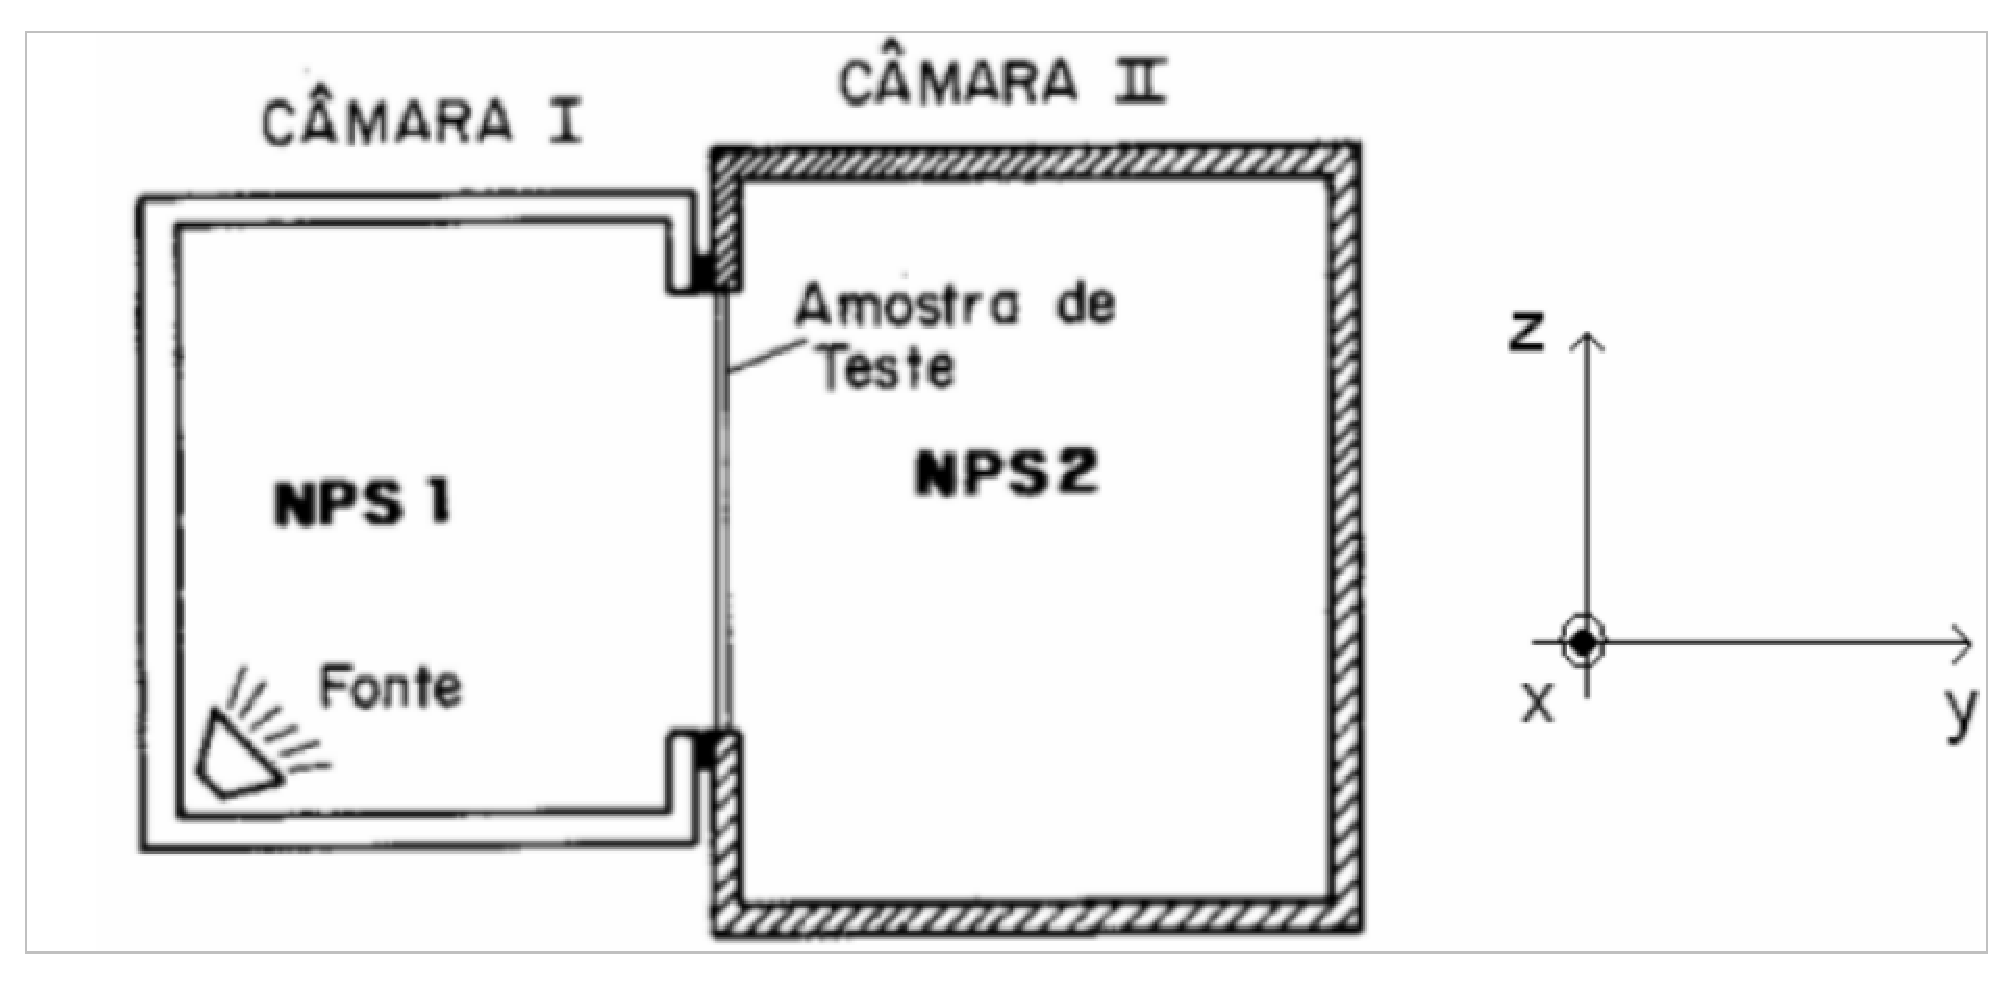
\includegraphics[scale=0.32]{imagem_3.eps}
	%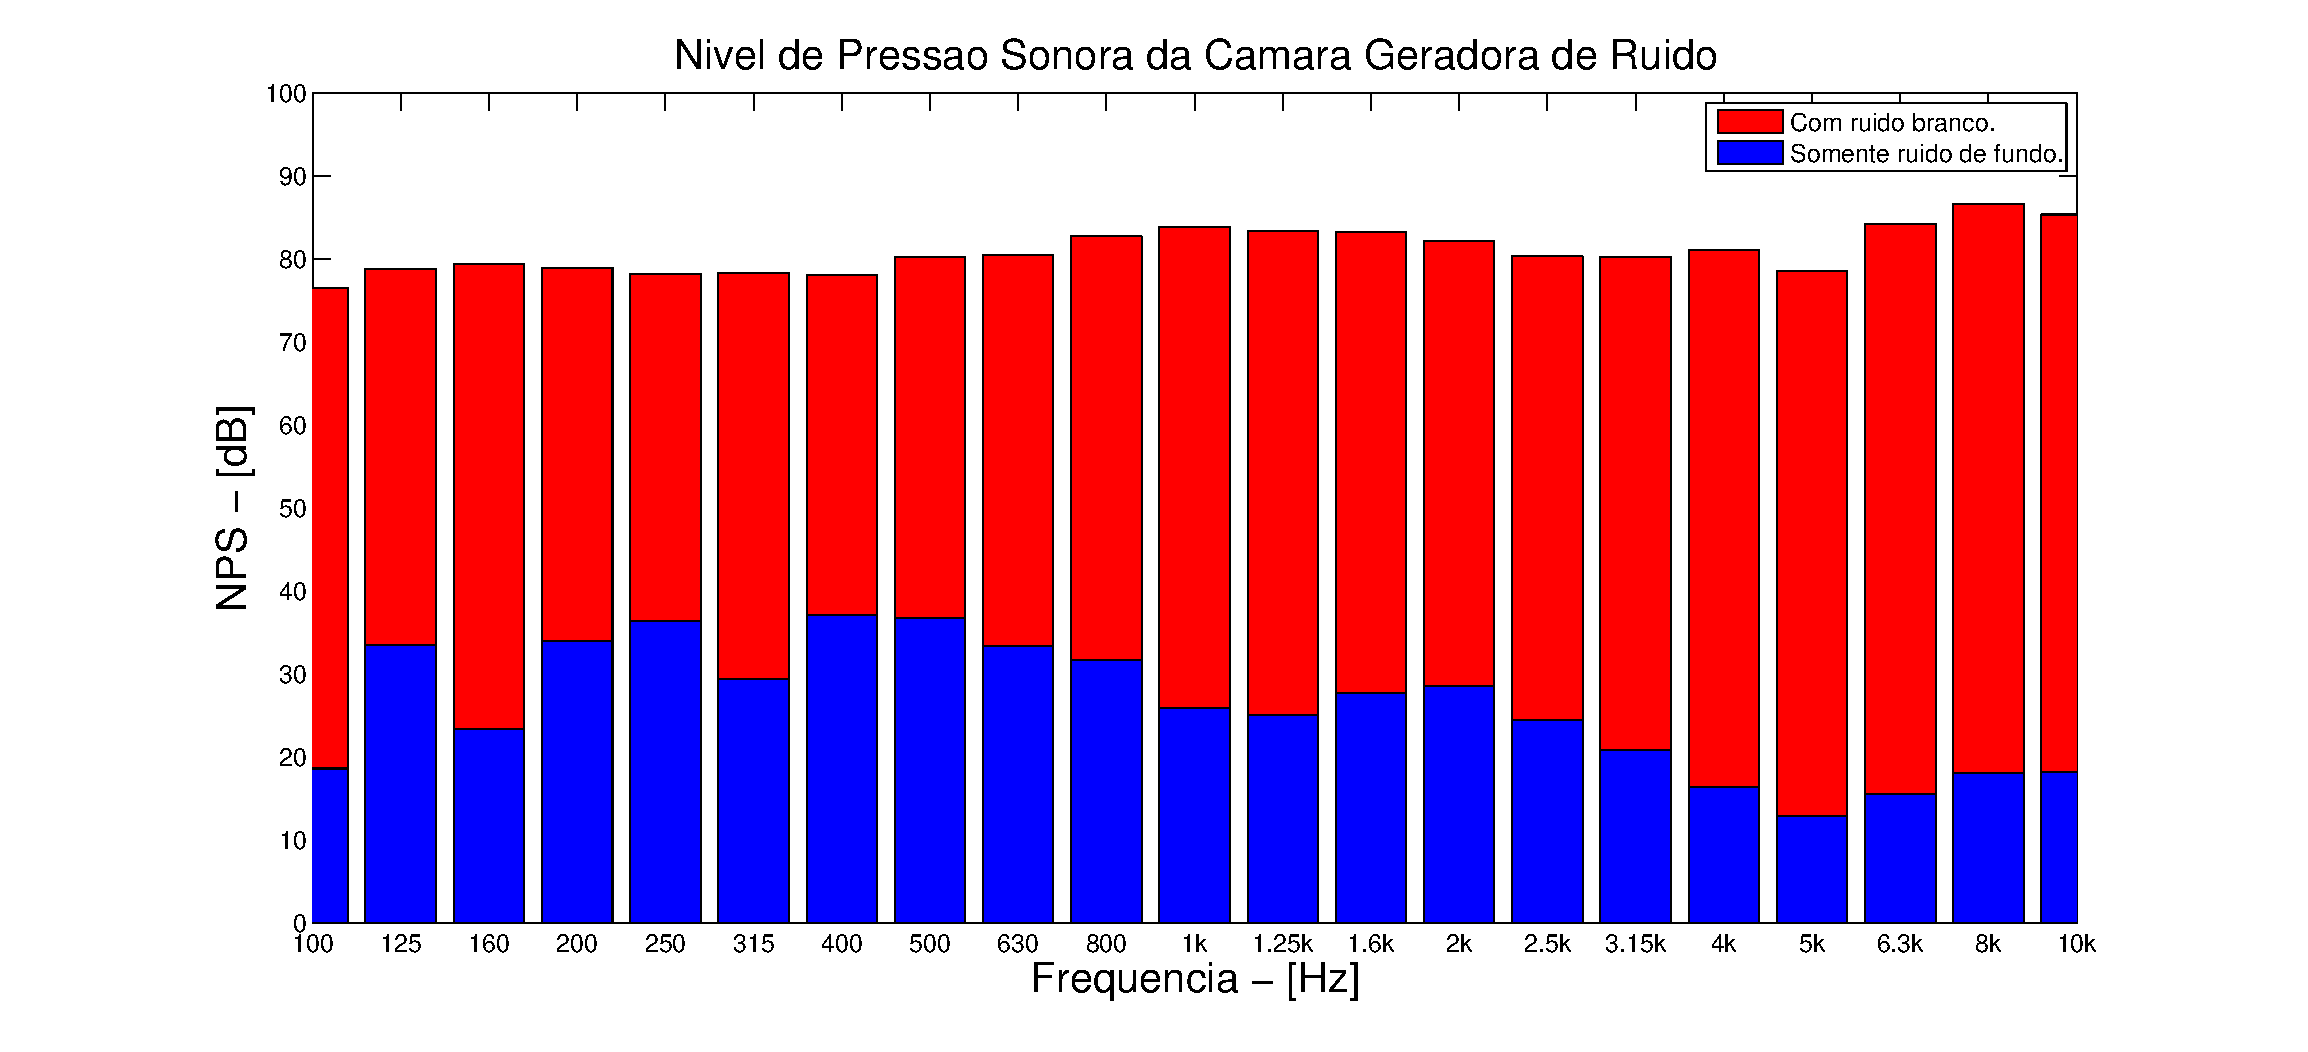
\includegraphics[width=40cm,height=40cm,keepaspectratio]{codigo/pressao_sonora_geradora.eps}
	\caption{Esquemático do acoplamento das camaras I e II. Fonte: \cite{silva2009simulaccao}}
	\label{experimento_1}
\end{figure}

\newpage
Segue as dimensões das câmaras I e II na figura \ref{experimento_2}.

\begin{figure}[h]
	\centering
	%\hspace{-4.5cm}
	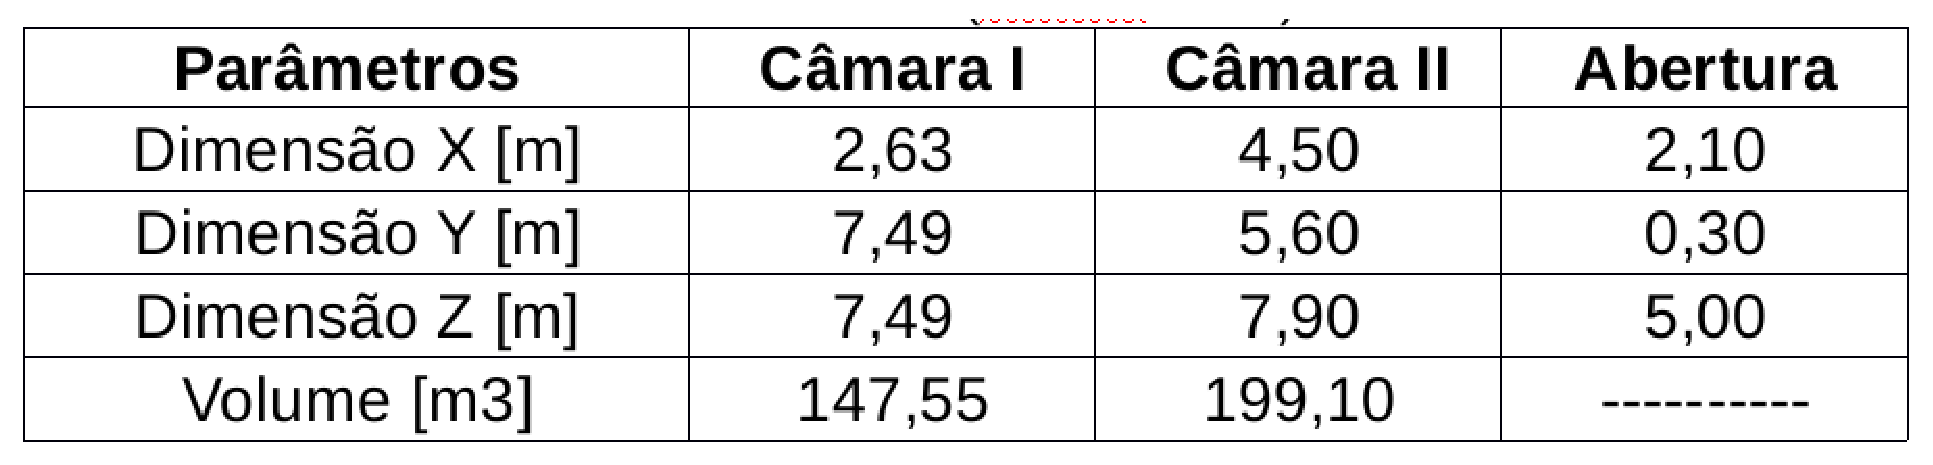
\includegraphics[scale=0.35]{imagem_4.eps}
	%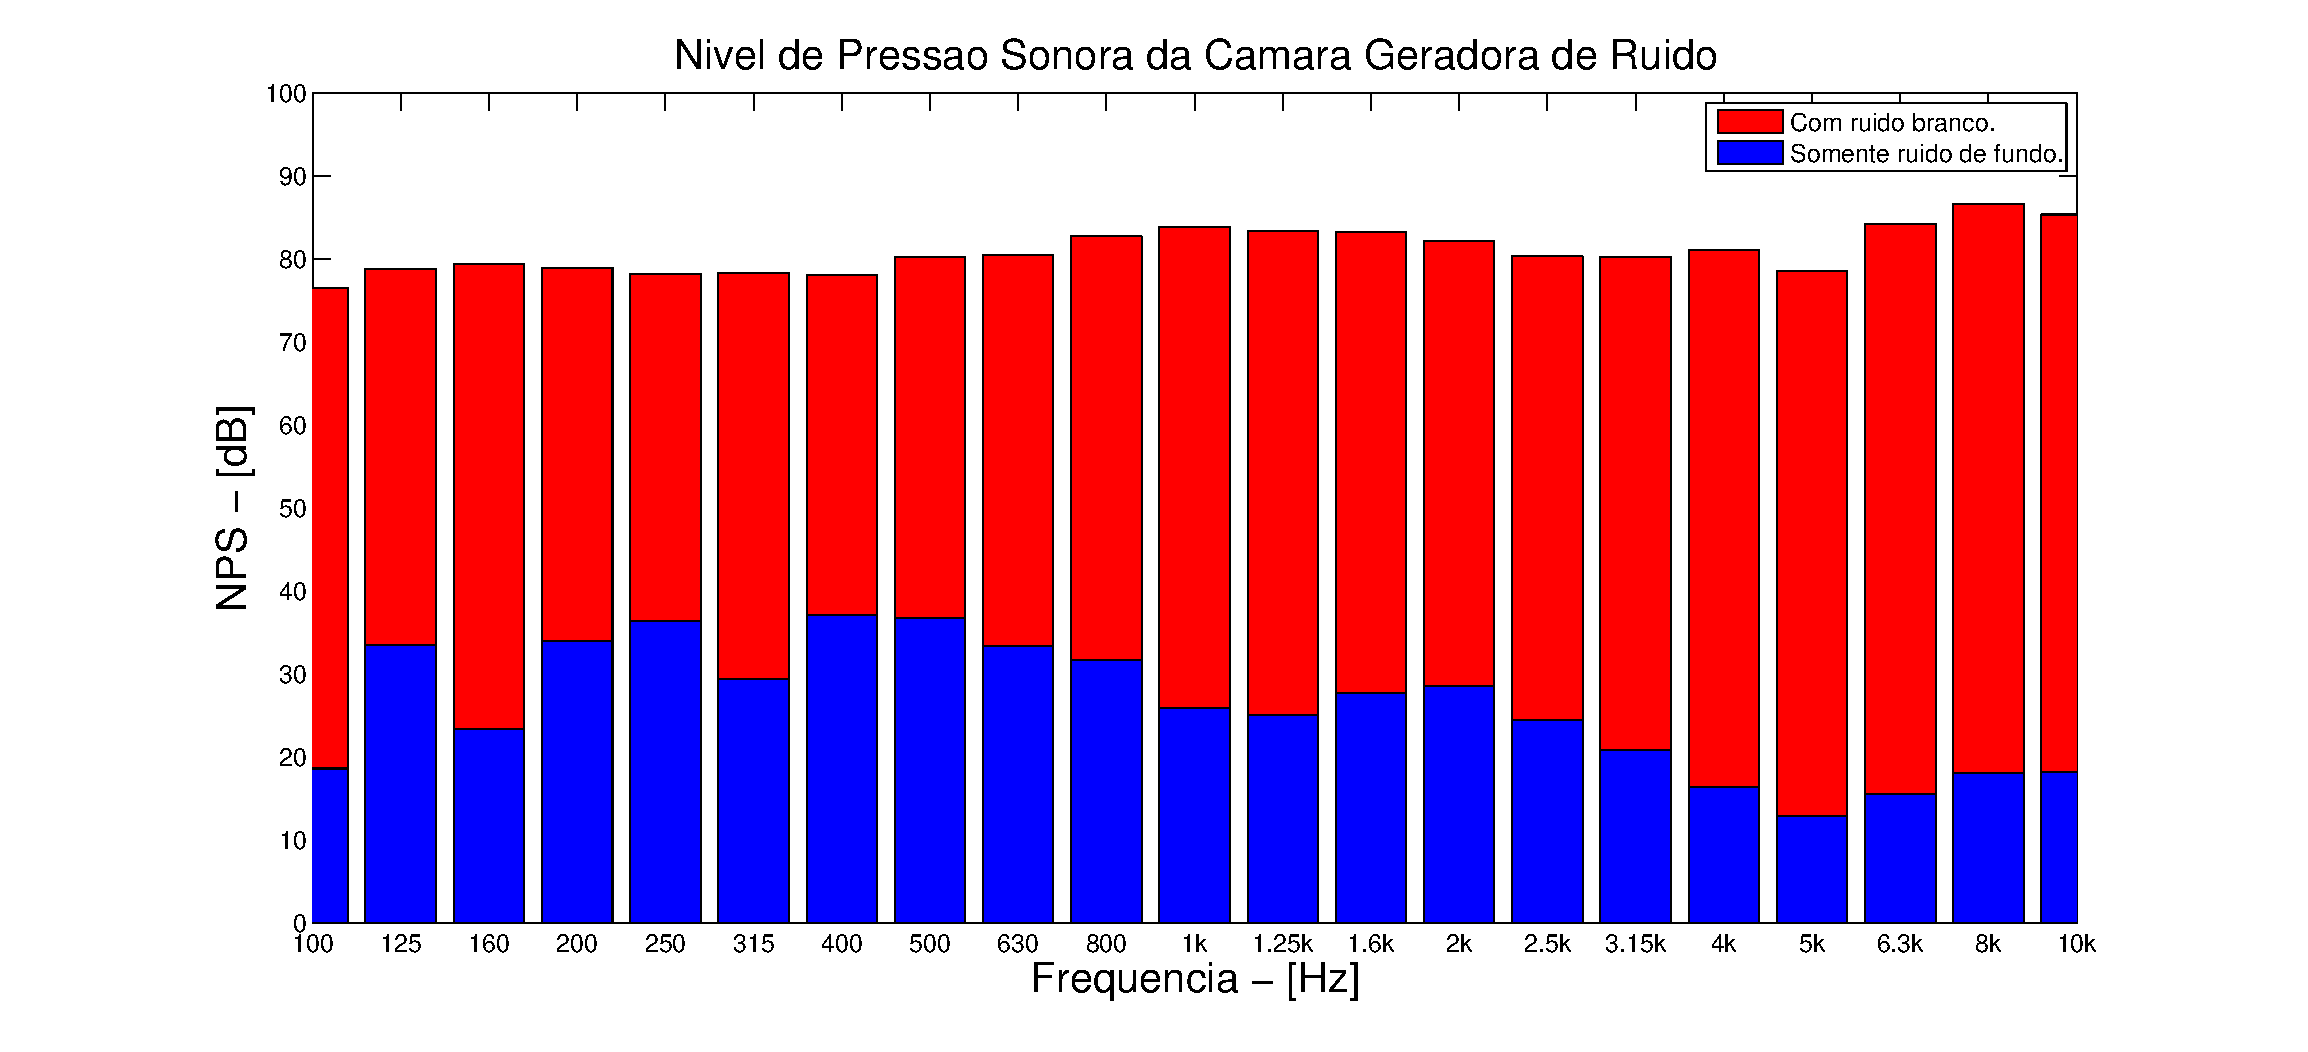
\includegraphics[width=40cm,height=40cm,keepaspectratio]{codigo/pressao_sonora_geradora.eps}
	\caption{Dimensões das câmaras I e II. Fonte: \cite{silva2009simulaccao}}
	\label{experimento_2}
\end{figure}

Segue os tempos de reverberação das câmaras I e II na figura \ref{experimento_3}.
\begin{figure}[h]
	\centering
	%\hspace{-4.5cm}
	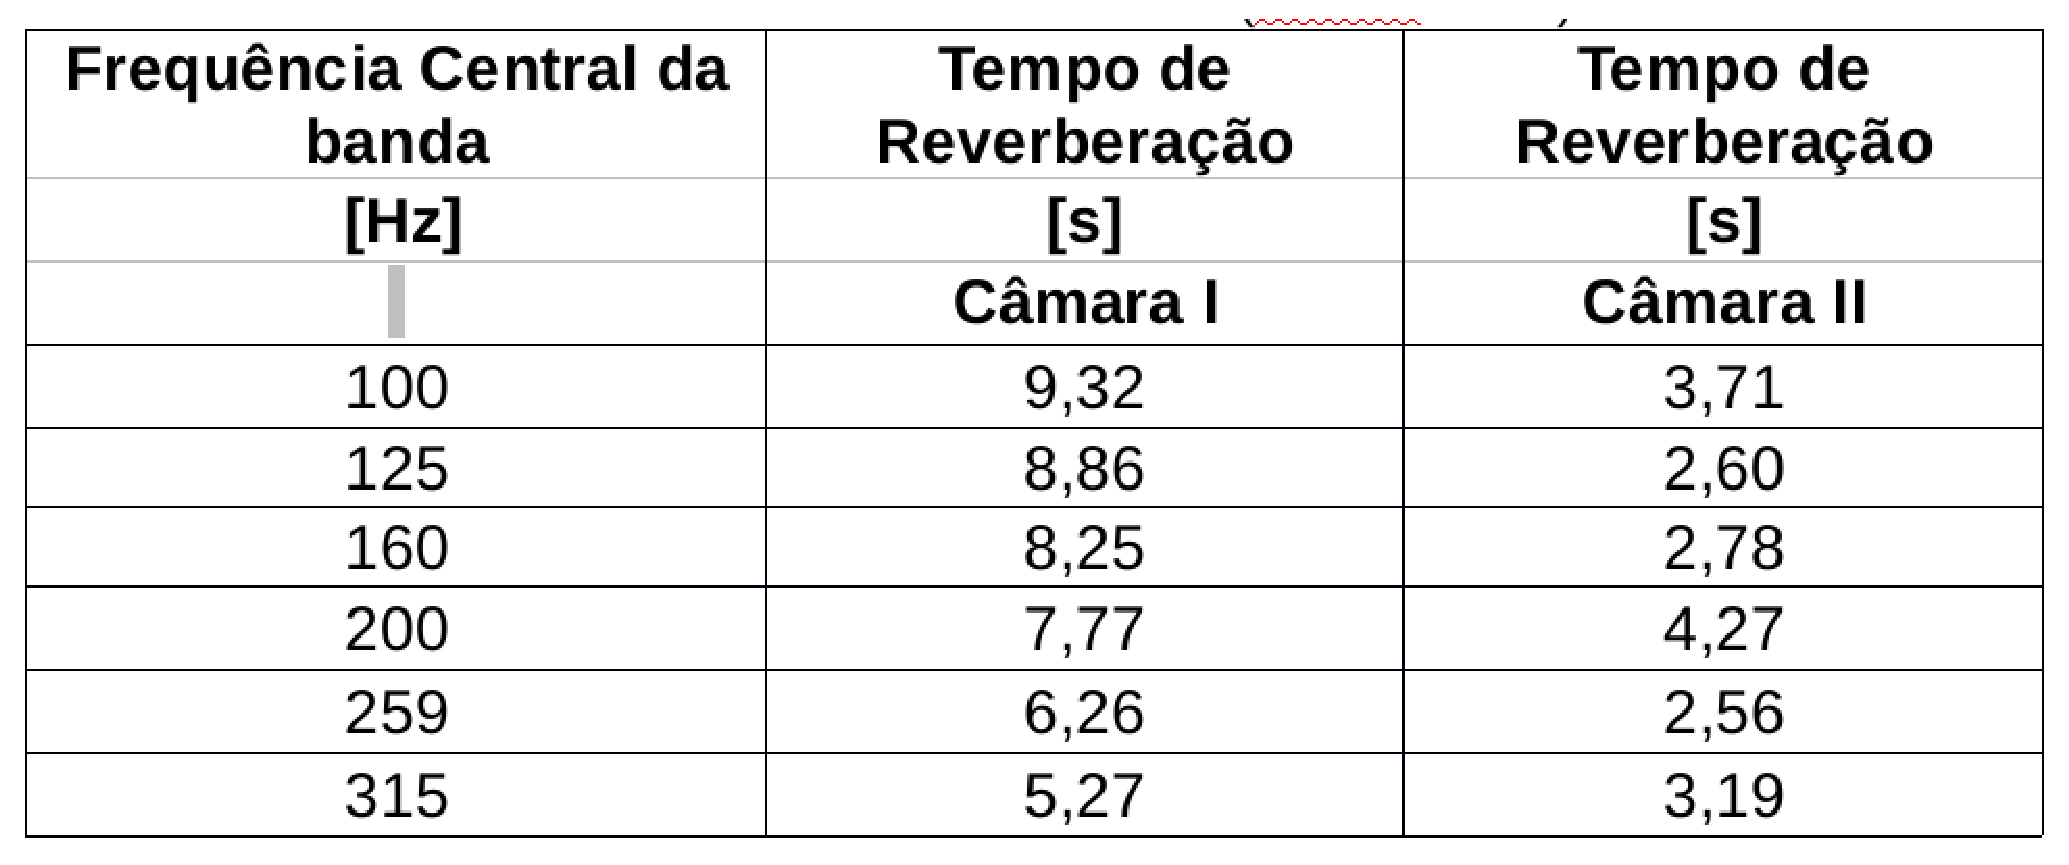
\includegraphics[scale=0.35]{imagem_5.eps}
	%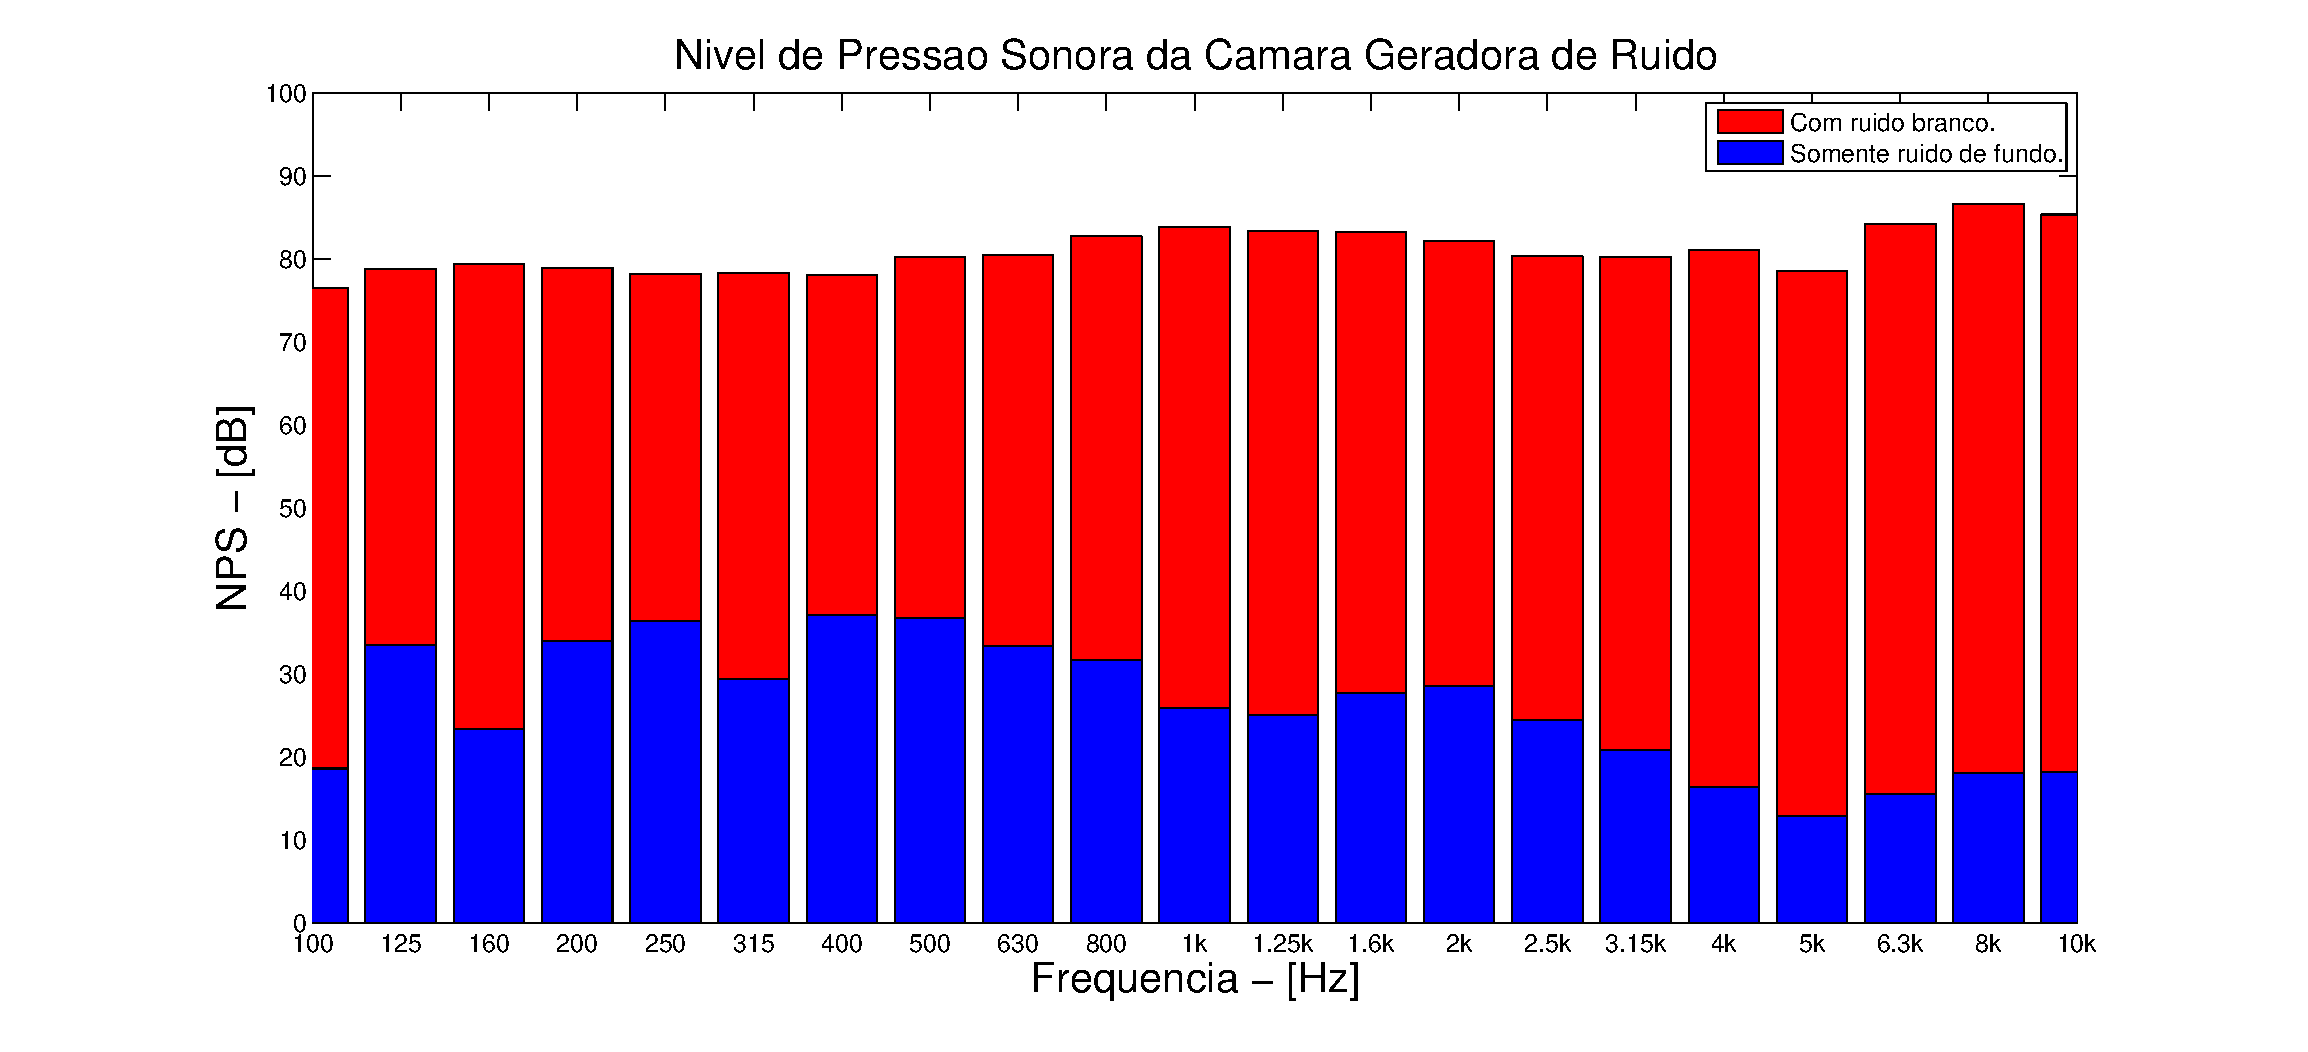
\includegraphics[width=40cm,height=40cm,keepaspectratio]{codigo/pressao_sonora_geradora.eps}
	\caption{Tempos de reverberação das câmaras I e II. Fonte: \cite{silva2009simulaccao}}
	\label{experimento_3}
\end{figure}

Segue disposição experimental da câmara I geradora na figura \ref{experimento_4}.


\chapter{Resultados}\label{resultados}

No que diz respeteito aos resultados do experimento abordado, foram consolidados o espectro de frequências do ruído branco e do ruído de fundo nas salas geradoras e receptoras respectivamente e, como resultado principal, foi extraído a perda de transmissão em relação as frequências por 2 métodos, o indireto (por comparação) e direto (por sabine, usando o tempo de reverberação da câmara).

\begin{figure}[h]
%\centering
\hspace{-4.5cm}
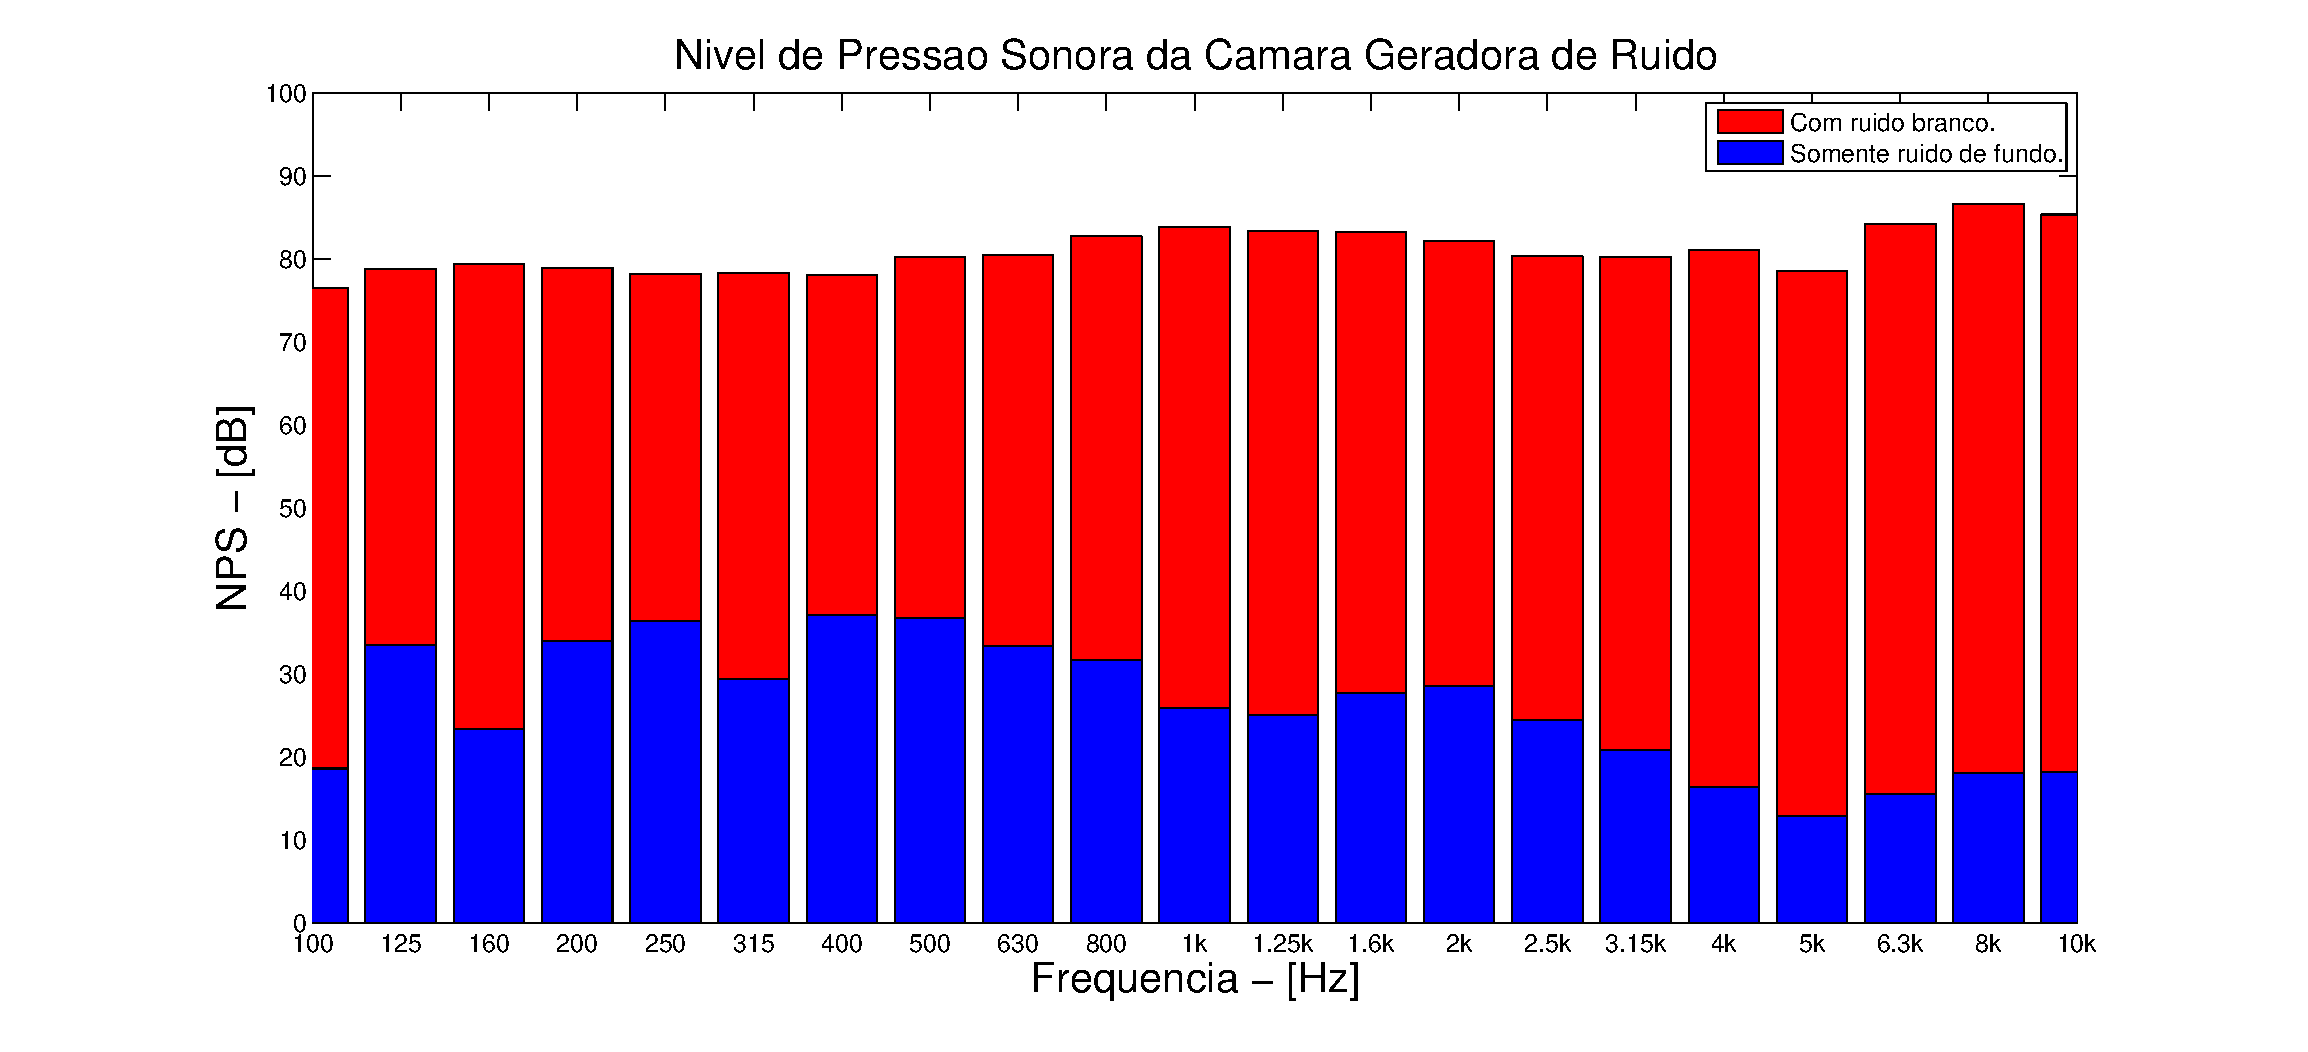
\includegraphics[scale=0.6]{codigo/pressao_sonora_geradora.eps}
%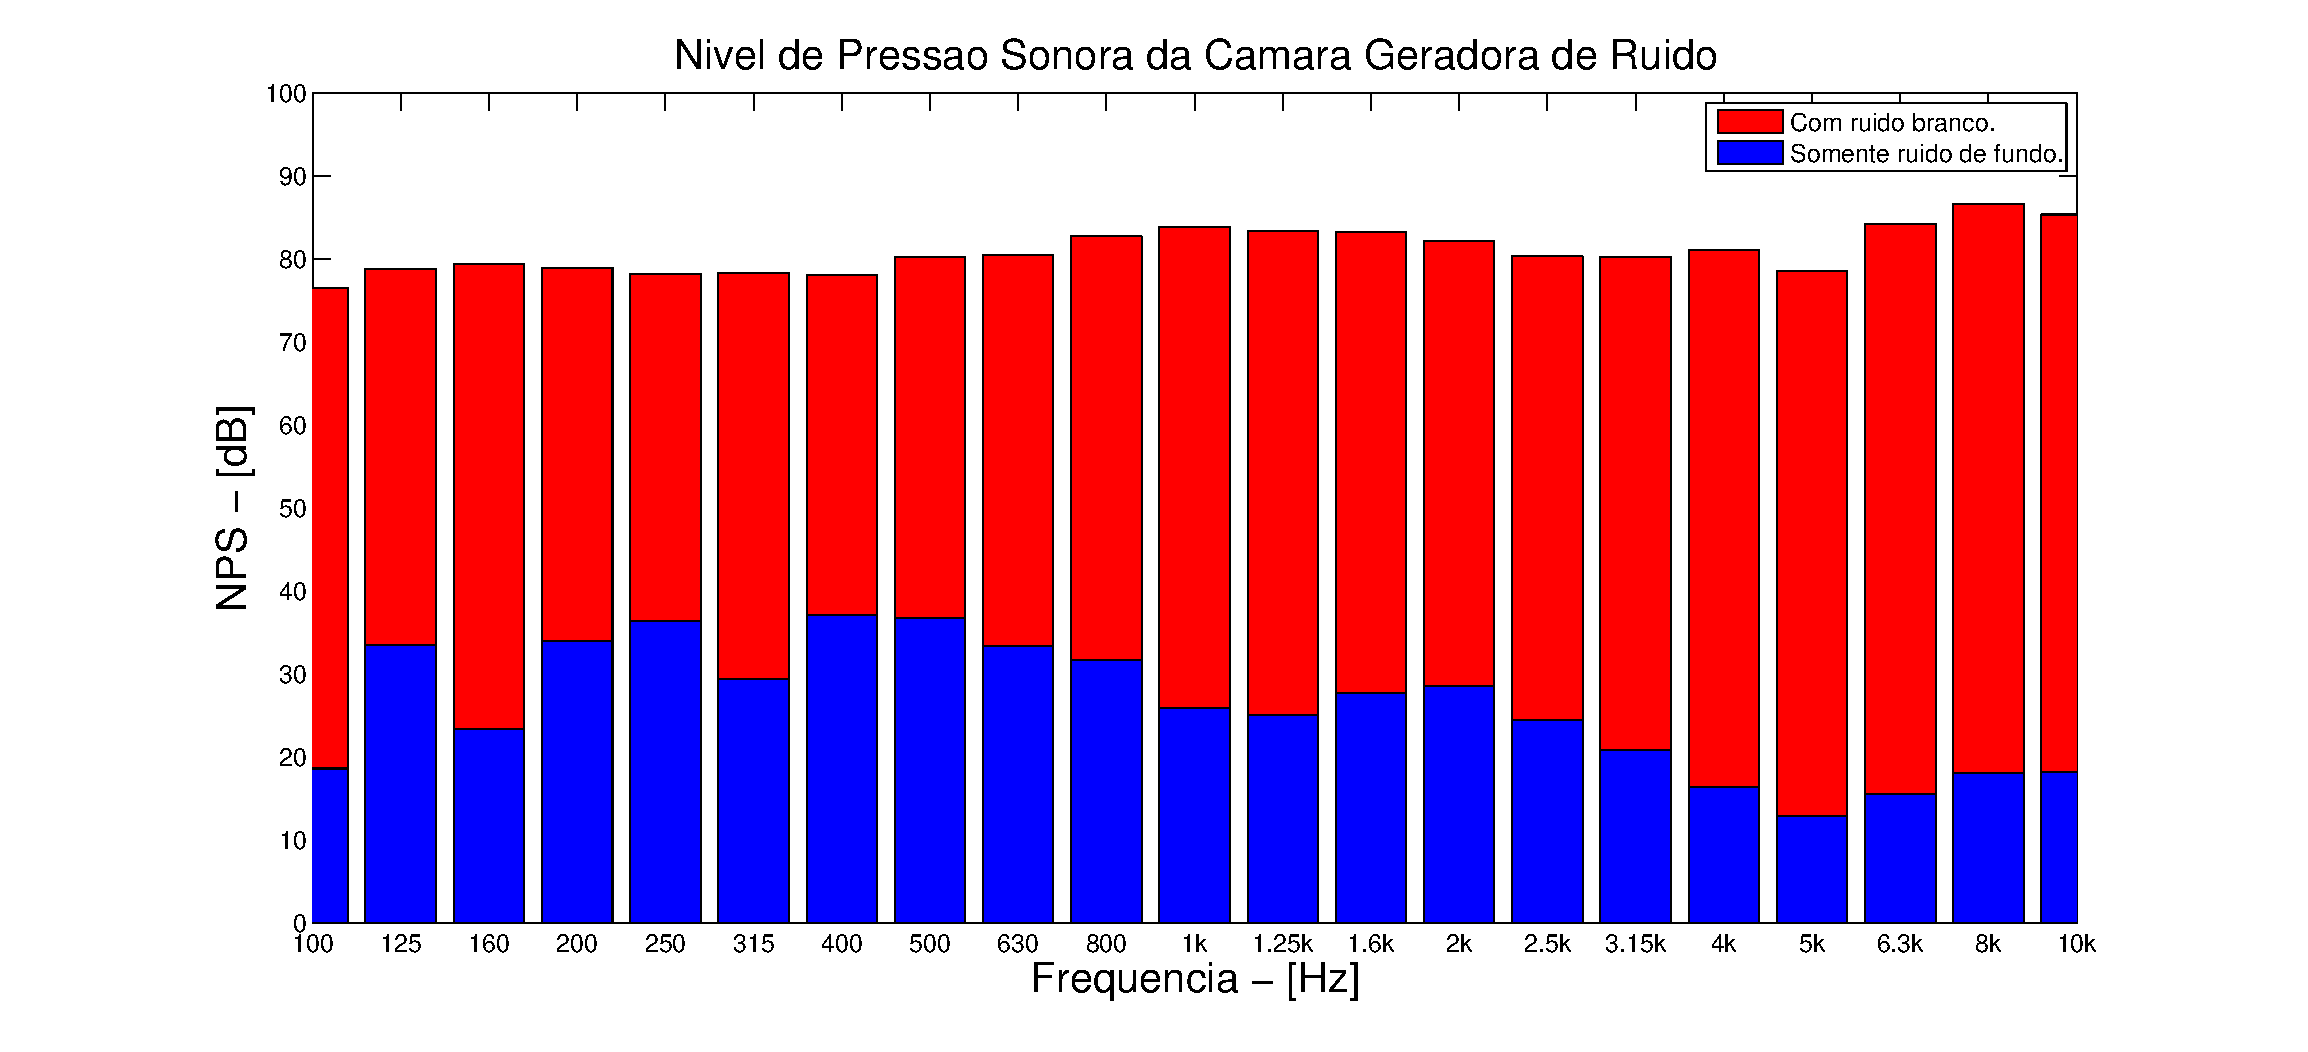
\includegraphics[width=40cm,height=40cm,keepaspectratio]{codigo/pressao_sonora_geradora.eps}
\caption{Níveis de pressão sonora na câmara geradora de ruído branco.}
\label{resultado_1}
\end{figure}

Diante do que é exposto no gráfico da figura \ref{resultado_1} é perceptível que o ruído branco se sobressaiu mais que 15 dB em relação ao ruído de fundo. Esse fato corrobora com uma medida sem necessidades de correção, pelo que é exposto em \cite{silva2009simulaccao}.

\newpage
\begin{figure}[h]
%\centering
\hspace{-4.5cm}
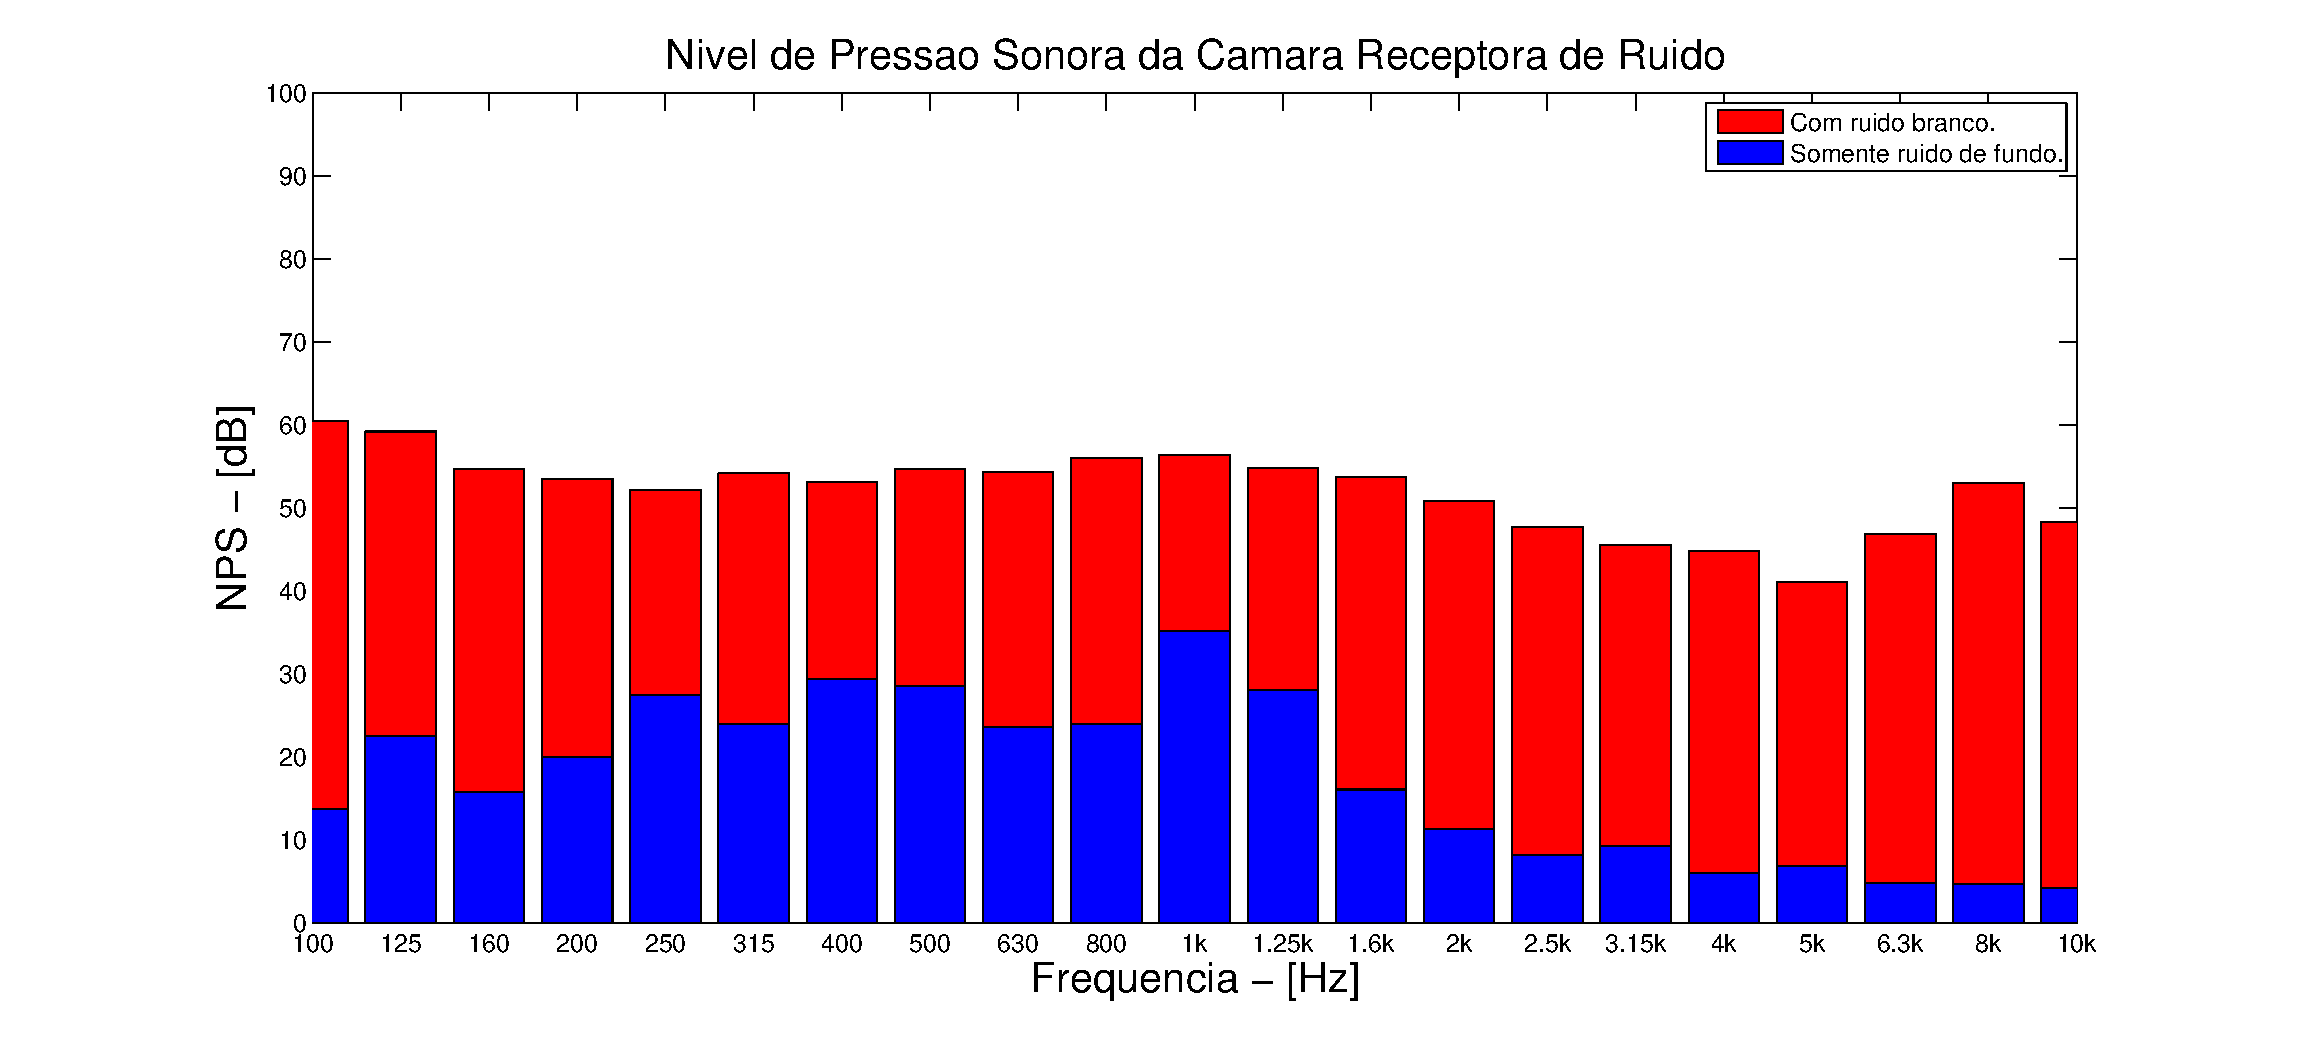
\includegraphics[scale=0.6]{codigo/pressao_sonora_receptora.eps}
\caption{Níveis de pressão sonora na câmara receptora de ruído branco.}
\label{resultado_2}
\end{figure}

Diante do que é exposto no gráfico da figura \ref{resultado_2} é perceptível que o ruído branco se sobressaiu mais que 15 dB em relação ao ruído de fundo. Esse fato corrobora com uma medida sem necessidades de correção, pelo que é exposto em \cite{silva2009simulaccao}.

\newpage
\begin{figure}[h]
%\centering
\hspace{-4.5cm}
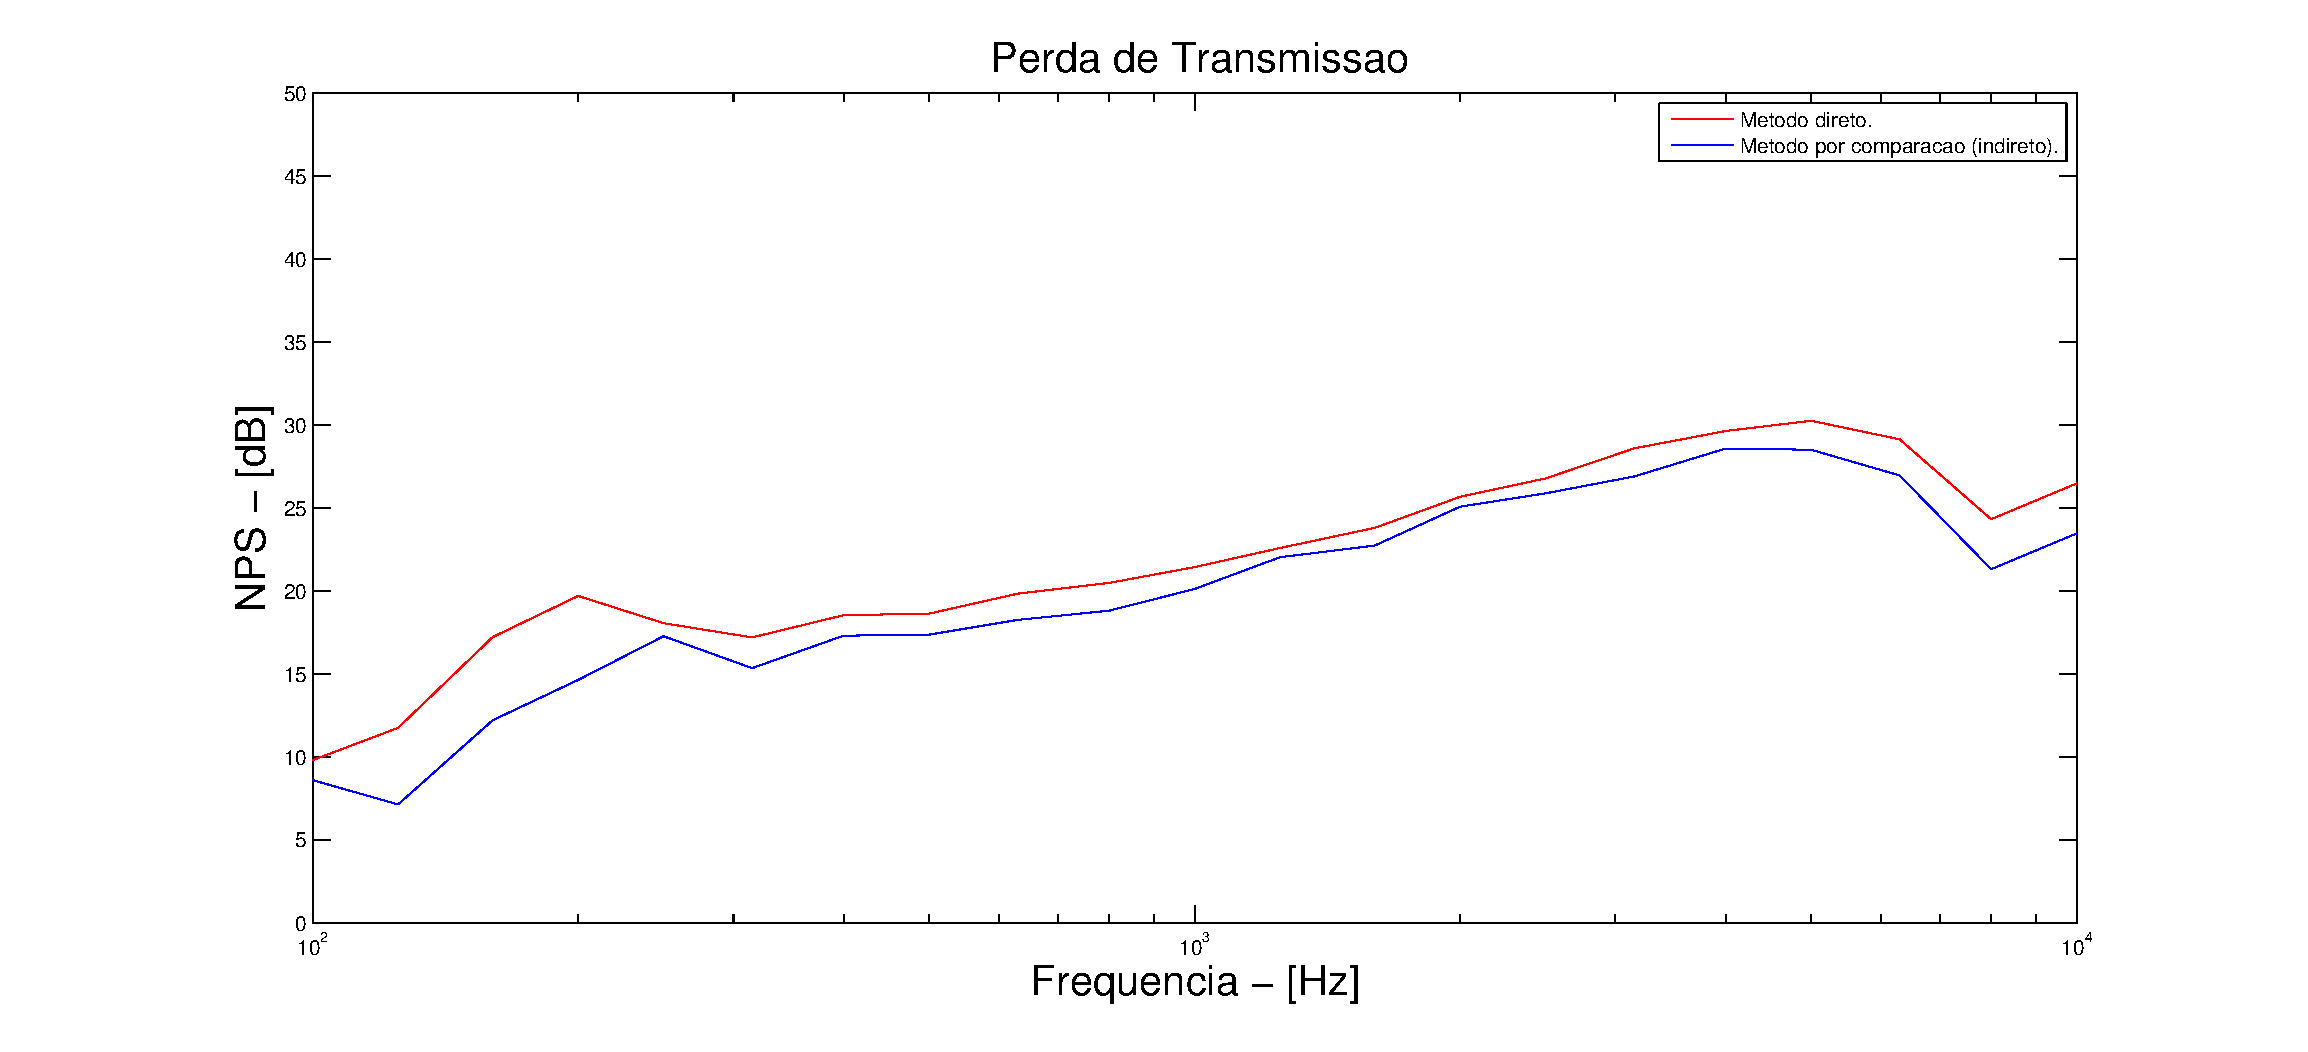
\includegraphics[scale=0.6]{codigo/perda_transmissao.eps}
\caption{Gráfico de perda de transmissão da placa de alumínio.}
\label{resultado_3}
\end{figure}

A figura \ref{resultado_3} mostra o resultado principal do experimento: a perda de transmissão em relação a frequência. É perceptível que, a medida que a placa é exposta para altas frequências, há uma perda maior. E esse fato corrobora com o que é medido pelo método indireto (feito por tempo de reverberação). As extremidades do gráfico, onde aparecem as curvas, dizem respeito ao regime elástico de comportamento, a parte linear diz respeito ao regime rígido da placa.


\chapter{Conclusões}\label{conclusoes}

O experimento descrito anteriormente reforçou as particularidades do uso da câmara de expansão e do ressonador de Helmholtz frente a perda de transmissão. Observa-se que o ressonador de Helmholtz atua como uma solução precisa e pontual, atuando em uma determinada frequência única. Ao contrário da câmara de expansão, que atua em uma faixa larga de frequência. No entanto esta última deve ser projetada para que os maiores níveis de atenuação ocorram nas frequências que deseja-se, caso contrário pode-se encontrar um anti-pico na curva e sua utilização não ter efeito nenhum de atenuação(1296 Hz, 2524 Hz e 3810 Hz).